%%
%% Journal extension of the PIWM conference paper.
%% "Physically Interpretable World Models via Weakly Supervised
%%  Representation Learning" (conference) -> journal version.
%%
%% This journal version extends the conference paper along three axes:
%%   (1) two new partially observable driving case studies
%%       -- simulated CarRacing and a real physical DonkeyCar;
%%   (2) physically interpretable encoding of the external road environment;
%%   (3) physically interpretable prediction of the road environment.
%%
\documentclass[preprint,12pt]{elsarticle}

\usepackage{amssymb}
\usepackage{amsmath}
\usepackage{amsthm}
\usepackage{graphicx}
\usepackage{subcaption}
\usepackage{booktabs}
\usepackage{algorithm}
\usepackage{algpseudocode}
\usepackage{siunitx}

\newtheorem{definition}{Definition}
\newtheorem{problem}{Problem}
\renewcommand{\algorithmicrequire}{\textbf{Input:}}
\renewcommand{\algorithmicensure}{\textbf{Output:}}

% Convenience macros for the factorized interpretable state.
\newcommand{\zv}{z^{v}}      % vehicle-relative state
\newcommand{\zr}{z^{r}}      % road-context state
\newcommand{\zstar}{z^{*}}   % interpretable state

\journal{Robotics and Autonomous Systems}

\begin{document}

\begin{frontmatter}

\title{Physically Interpretable World Models for Partially Observable
       Driving: Encoding and Predicting the Road Environment under
       Weak Supervision}

\affiliation[uf]{organization={Trustworthy Engineered Autonomy (TEA) Lab,
                               University of Florida},
               city={Gainesville},
               state={Florida},
               country={USA}}

%% ---------------------------------------------------------------
\begin{abstract}
Learning predictive models from high-dimensional sensory observations is
fundamental for safe autonomous cyber-physical systems, yet the latent
representations of standard world models lack physical interpretability.
Our prior conference work introduced the Physically Interpretable World Model
(PIWM), which aligns latent representations with physical quantities and
constrains their temporal evolution through partially known dynamics, trained
under distribution-based weak supervision derived from realistic sensing
pipelines.
That formulation implicitly assumes that the system's physical state provides a
complete Markov description of the task, a condition that holds for
fully observable benchmarks such as CartPole and Lunar Lander but fails for
realistic driving.
Two vehicles with identical position, heading, and speed can follow divergent
futures when the road geometry ahead differs, because a standard vehicle state
encodes nothing about the lane or the vehicle's relationship to it.
Driving is therefore \emph{partially observable}: the world model must reason
not only about the vehicle but about the external road environment, which is
neither part of the vehicle state nor fully visible from an onboard camera.

This article extends PIWM to partially observable driving along three axes.
First, we move beyond the fully observable benchmarks to two new
partially observable case studies: a simulated top-down \emph{CarRacing}
environment and a \emph{real, physical DonkeyCar} platform driven on a
laboratory track.
Second, we introduce a physically interpretable \emph{encoding} of the road
environment: the interpretable latent is factorized into a vehicle-relative
component and a road-context component (lateral deviation, vehicle--road
heading error, and road curvature) that is inferred from images even when the
road ahead is only partially visible.
Third, we introduce a physically interpretable \emph{prediction} of the road
environment: a split-dynamics model couples a learnable bicycle kinematic model
for the vehicle with a structured, geometry-driven transition that forecasts how
the road context evolves.
On the real DonkeyCar, ground-truth road context is available only at training
time through external track localization and is withheld at test time, so the
model must recover and roll out road context from onboard images alone.
Across the original benchmarks, simulated CarRacing, and the physical DonkeyCar,
PIWM with factorized state and split dynamics substantially outperforms
data-driven and physics-informed baselines at long prediction horizons,
demonstrating that physically grounded driving world models must both encode and
predict the external road environment, not merely the vehicle state.
\end{abstract}

\begin{keyword}
physically interpretable world models \sep partial observability \sep
autonomous driving \sep road-context encoding \sep road prediction \sep
bicycle dynamics \sep weak supervision \sep trajectory prediction
\end{keyword}

\end{frontmatter}

%% ==============================================================
\section{Introduction}\label{sec:intro}
%% ==============================================================

Accurate and robust trajectory prediction from high-dimensional sensor data
is a foundational challenge for autonomous cyber-physical systems (CPS).
Modern \emph{world models}~\cite{ha2018world} address this challenge by
encoding observations into compact latent representations and predicting their
temporal evolution, a paradigm that has proven effective for long-horizon
prediction, planning, and control~\cite{micheli2022transformers,
hafner2023mastering, seo2023masked}.
Despite strong empirical performance, the latent states of these models
typically lack a clear connection to the underlying physical state of the
system.
In safety-critical settings such as autonomous driving and robotics, this
opacity limits trustworthiness: without interpretable states, it is difficult
to detect unsafe future configurations, diagnose prediction failures, or apply
formal safety-monitoring techniques~\cite{hasan2015formal, katz2022verification,
alshiekh2018safe}.

Our prior conference work introduced the Physically Interpretable World Model
(PIWM)~\cite{piwm_conf}, a framework that aligns latent representations with
physical quantities and constrains their temporal evolution through a partially
known dynamics model.
PIWM defines physical interpretability through two complementary properties:
the latent state must correspond to meaningful physical variables (state
semantics), and its temporal evolution must follow physically consistent
dynamics (temporal correctness).
A key feature of PIWM is \emph{distribution-based weak supervision}: rather than
requiring precise ground-truth state labels, the method accepts state estimates
in the form of sample distributions, as naturally produced by real-world sensing
pipelines such as GPS or radar.
Experiments on CartPole, Lunar Lander, and DonkeyCar demonstrated that
PIWM recovers accurate physical parameters and achieves long-horizon prediction
accuracy well beyond data-driven baselines.
A systematic comparison of intrinsic versus extrinsic architectures and
continuous versus discrete latent spaces showed that an extrinsic architecture
with a quantized (VQ-based) latent yields the most robust and physically grounded
representations.

\subsection*{The challenge: driving is partially observable}

Applying PIWM to realistic driving exposes a fundamental limitation of the
original formulation, and motivates the extensions in this article.
On CartPole and Lunar Lander, the system state completely specifies what will
happen next: the dynamics are fully observable and Markov, so a world model that
tracks the vehicle (or pole, or lander) state captures everything relevant to the
future.
Driving is different.
Consider two vehicles with identical position, heading, and speed.
If one is approaching a tight curve while the other is on a straight segment,
their future trajectories diverge substantially even under the same control
inputs.
The vehicle's physical state $x_t = (x, y, \psi, v)$ does not capture this
difference.
The missing information is the \emph{road context}: the shape of the lane ahead
(its curvature) and the vehicle's lateral and angular relationship to it, none of
which is part of any standard vehicle-state representation.
As a result, the vehicle state alone is \emph{non-Markov} with respect to future
motion: two identical states lead to different futures depending on the
unobserved road geometry.
Applying the original PIWM formulation to such tasks implicitly treats the
system as fully observable when it is not, causing the dynamics model to learn an
underdetermined, ill-posed mapping.

This challenge has two distinct facets, and overcoming each requires a separate
mechanism.
\emph{(i) The road environment must be encoded.}
The relevant road context is not given as a clean state vector; it is latent in
the pixels and, for a forward-facing camera, only partially visible at any
instant.
A physically interpretable driving world model must therefore \emph{infer} the
geometry of the surrounding road from raw images, and represent it in physically
meaningful terms rather than as opaque features.
\emph{(ii) The road environment must be predicted.}
Long-horizon rollout requires anticipating how the road context itself evolves as
the vehicle advances: the lane that is far ahead now becomes the lane the vehicle
is on a few steps later.
A world model that predicts only the vehicle state, treating the road as static
or as noise, accumulates error rapidly because it cannot anticipate the geometry
it is about to enter.
Predicting the road, like encoding it, should be physically interpretable so that
the forecasted environment can be inspected, trusted, and monitored.

\looseness=-1
These two facets, encoding and predicting the external environment, are precisely
what distinguishes a driving world model from the vehicle-centric formulation of
the conference paper, which modeled only the state of the controlled body.
They are also why partial observability cannot be papered over by simply adding
capacity to a black-box predictor: the missing variable is structured, physical,
and causally upstream of the vehicle's future, so it deserves an explicit,
physically grounded treatment.

\subsection*{Our approach}

We resolve partial observability by reformulating the interpretable state as a
structured composition of two complementary components.
The \emph{vehicle-relative state} $\zv$ captures the ego vehicle's displacement
and heading change expressed in a local reference frame anchored at the beginning
of each prediction window; this representation removes dependence on global
coordinates and improves transferability across trajectories.
The \emph{road-context state} $\zr$ captures task-relevant environmental
structure: the cross-track error (lateral deviation from the lane center), the
vehicle--road heading error, and the local road curvature.
Together, $(\zv, \zr)$ form a Markov description of the driving task, restoring
the validity of the predictive world-model framework.
The vehicle-relative component is governed by a learnable bicycle kinematic
model, whose parameters (e.g., the effective wheelbase) are unknown and recovered
during training.
The road-context component is governed by a structured, geometry-driven
transition that reflects the slow, conservative evolution of lane variables.
This split-dynamics formulation provides appropriate inductive biases for each
component and decouples the faster-varying vehicle motion from the
slower-varying road context.

We validate the extended formulation in two new partially observable driving
environments.
In \textbf{CarRacing}, a top-down simulated racing environment, the road geometry
is present in the image but absent from the vehicle state; the model must learn to
infer and exploit road-context information from raw pixels.
On the physical \textbf{DonkeyCar} platform, a real RC-scale car observes its
environment through a front-facing camera and drives on a laboratory track.
During training, an external localization system provides ground-truth road
context as a privileged signal; at test time this signal is withheld, and the
model must infer and roll out road context solely from the onboard front-facing
image stream.
This setup tests whether the factorized representation learned under privileged
supervision transfers to the more challenging unaided real-world deployment
setting.
Across both environments and at prediction horizons of up to 100 steps, PIWM with
factorized state and split dynamics substantially outperforms data-driven
baselines and physics-informed alternatives.

\subsection*{Contributions}

This journal article substantially extends the conference version~\cite{piwm_conf}
along three axes, which constitute its three contributions.

\begin{enumerate}
    \item \textbf{Two partially observable driving case studies.}
    We move PIWM beyond the fully observable benchmarks of the conference paper
    to two new driving environments that are genuinely partially observable:
    a simulated top-down \emph{CarRacing} track and a \emph{real, physical
    DonkeyCar} platform driven on a laboratory track under onboard-camera
    observation.
    We formally characterize partial observability in driving, showing that the
    vehicle state is non-Markov with respect to future trajectory, and use these
    two case studies to demonstrate the practical consequences and the benefit of
    the proposed treatment.

    \item \textbf{Physically interpretable encoding of the road environment.}
    Unlike the conference formulation, which modeled only the controlled body's
    state, we model the \emph{external environment}.
    We introduce a factorization of the interpretable latent into a
    vehicle-relative component $\zv$ and a road-context component $\zr$, where
    $\zr$ comprises physically meaningful descriptors of the road (cross-track
    error, vehicle--road heading error, and curvature).
    We show how to infer $\zr$ from images using temporal context, including the
    forward-camera case where the road ahead is only partially visible, and how
    privileged supervision available only at training time can be used to learn
    this encoding.

    \item \textbf{Physically interpretable prediction of the road environment.}
    We introduce a split-dynamics model that not only rolls out the vehicle with
    a learnable bicycle kinematic model, but also \emph{forecasts the road
    context} with a structured, geometry-driven transition.
    The predicted road context is itself physically interpretable, so the
    forecasted environment, not just the forecasted vehicle, can be inspected and
    monitored.
    We show that predicting the road, rather than treating it as static, is what
    enables stable long-horizon prediction under partial observability.
\end{enumerate}

\noindent
Throughout, we precede the technical development of each extension with the
specific challenge and motivation that makes it necessary, in keeping with the
two facets of partial observability identified above.

The remainder of this article is organized as follows.
Section~\ref{sec:related} surveys related work.
Section~\ref{sec:preliminaries} reviews background on autonomous CPS, world
models, and physical interpretability.
Section~\ref{sec:problem} formalizes the partial observability problem in driving
and introduces the factorized state.
Section~\ref{sec:architecture} presents the PIWM architecture, the road-context
encoder (Section~\ref{sec:encoding}), and the road-context predictor
(Section~\ref{sec:prediction}).
Section~\ref{sec:experiments} describes the experimental setup, and
Section~\ref{sec:results} reports results on the benchmarks, CarRacing, and the
real DonkeyCar.
Section~\ref{sec:discussion} discusses implications and limitations, and
Section~\ref{sec:conclusion} concludes.


%% ==============================================================
\section{Related Work}\label{sec:related}
%% ==============================================================

We organize the discussion into five threads relevant to physically interpretable
world modeling under partial observability: trajectory prediction and safe forecasting
(Section~\ref{sec:rw_traj}), representation learning for dynamical systems
(Section~\ref{sec:rw_repr}), world models (Section~\ref{sec:rw_wm}),
physics-informed and interpretable learning (Section~\ref{sec:rw_phys}), and
partial observability, privileged learning, and road structure
(Section~\ref{sec:rw_po}).
We close each thread by positioning PIWM against it.

\subsection{Trajectory Prediction and Safe Forecasting}\label{sec:rw_traj}

Predicting future motion is central to safe planning and
control~\cite{fridovich2020confidence}.
Classical predictors propagate a low-dimensional state with hand-specified
models: constant-velocity and Kalman-filter formulations for vehicle
motion~\cite{ammoun2009real}, and Hamilton--Jacobi reachability for sets of
reachable states with formal guarantees~\cite{li2021prediction,
nakamura2023online, muthali2023multi}.
These methods are transparent and certifiable, but they require an explicit
dynamical model and a low-dimensional state, and they scale poorly to
high-dimensional camera observations.

Learning-based predictors instead forecast directly from data.
Social-pooling and generative sequence models capture multi-agent
interaction~\cite{alahi2016social, gupta2018social, wen2022social}, while graph-
and attention-based models such as Trajectron++ achieve strong forecasting by
conditioning on scene graphs and high-definition maps~\cite{salzmann2020trajectron++}.
Hybrid schemes embed classical filters inside learned models, as in learned
Kalman filtering~\cite{revach2022kalmannet}.
These models, however, depend on handcrafted scene representations or HD-map
annotations that are unavailable in many settings~\cite{itkina2023interpretable,
hsu2023interpretable}, and their internal states carry no physical meaning.

A parallel line equips predictors with reliability guarantees without altering
the predictor itself: conformal prediction and calibrated forecasting bound error
or coverage~\cite{lindemann2023conformal, lu2024towards, ruchkin2022confidence,
cleaveland2022risk}; statistical model checking and predictive monitoring estimate
the probability of property violations~\cite{qin2022statistical, zarei2020statistical,
cairoli2021neural, waga2022dynamic}; and runtime and misbehavior monitors flag
unsafe behavior online~\cite{stocco2020misbehaviour, ma2020stlnet, mao2024safe,
mao2025safe}.
These techniques are complementary to ours: they wrap a predictor with guarantees
but do not make its latent state physically meaningful.
Compared with this body of work, PIWM learns interpretable representations
directly from raw images under weak supervision, without handcrafted scene
representations or test-time state labels, so that the forecast itself, both the
vehicle and the road around it, can be inspected.

\subsection{Representation Learning for Dynamical Systems}\label{sec:rw_repr}

Compact latent representations underpin learning from high-dimensional
observations, from classical autoencoders~\cite{Hinton06} to variational
autoencoders (VAEs)~\cite{kingma2013auto}, but standard objectives impose no
physically meaningful structure.
A large literature seeks more structured latents by encouraging
disentanglement~\cite{higgins2017beta, kim2018disentangling, chen2018isolating},
causal structure~\cite{yang2021causalvae, scholkopf2021toward}, or object-centric
and slot decompositions~\cite{mosbach2025soldslotobjectcentriclatent}.
Discrete VQ-VAEs regularize the latent through a learned
codebook~\cite{van2017neural, razavi2019generating}; PIWM builds on this
quantization but, unlike it, ties codebook components to physical values.
These methods improve organization or modularity, yet none guarantees
correspondence to measurable physical quantities.

Closer to physical grounding, several models steer latents toward physics.
GOKU-Net restricts latent variables to plausible physical ranges without binding
them to specific quantities~\cite{linial_generative_2021}; SPARTAN produces
semantically structured outputs but incorporates neither known dynamics nor
action-conditioned prediction~\cite{lei2024spartan}; Deep Variational Bayes
Filters add latent state-space dynamics to VAEs~\cite{karl2016deep} but, absent
physical supervision, do not recover interpretable variables; and continuous-time
models such as Neural ODEs learn smooth but uninterpretable latent
dynamics~\cite{chen2018neural}.
Representation learning specialized for pixel-based control improves downstream
performance~\cite{tomar2021learningrepresentationspixelbasedcontrol} while again
leaving the latent opaque.
Compared with these approaches, PIWM explicitly aligns latent dimensions with
named physical quantities of both the vehicle and the surrounding road, and
constrains their evolution with known physics under only weak, distribution-based
supervision.

\subsection{World Models}\label{sec:rw_wm}

World models learn latent dynamics for imagination-based planning and control.
The Dreamer and PlaNet line learns recurrent latent state-space models from
pixels~\cite{hafner2019learning, hafner2020mastering, hafner2023mastering};
transformer- and masked-prediction world models improve sample efficiency and
long-horizon fidelity~\cite{micheli2022transformers, seo2023masked,
wu2023daydreamer}; and a range of variants explore alternative latent
factorizations~\cite{ha2018world, zhang2021world, zhao2024decomposed}.
These models excel empirically but learn latent spaces with no clear physical
meaning, which limits inspection and safety monitoring.

For driving, recent world models predict rich structured futures such as 3D
occupancy grids or rendered scenes~\cite{zheng2024occworld, min2023uniworld,
yan2024renderworld, zuo2024gaussianworld}, improving forecasting realism but still
without aligning the internal state to physical variables, and at substantial
annotation and compute cost.
Neuro-symbolic world models improve generalization but require predefined symbolic
inputs unavailable from raw sensors~\cite{balloch2023neuro, liang2024visualpredicator}.
The closest prior work, Vid2Param, recovers physical parameters from
video~\cite{asenov2019vid2param} but requires full supervision and provides no
explicit world model for long-horizon rollout.
Compared with these approaches, PIWM recovers physical state under weak
supervision and rolls it forward through interpretable dynamics, and, new in this
article, it does so for the external road environment, not only the controlled
body.

\subsection{Physics-Informed and Interpretable Learning}\label{sec:rw_phys}

A complementary thread injects physics directly into learning.
Sparse identification of nonlinear dynamics and differentiable-physics or
end-to-end system identification recover governing equations or
parameters~\cite{BRUNTON2016710, de2018end, yao2024marrying}, while
physics-informed neural networks embed differential constraints in the
loss~\cite{cai2021physics, ZHONG2023115664}.
Within world modeling, physical priors have been added as bounds on states and
actions~\cite{tumu2023physics, sridhar2023guaranteed}, physics-aware
losses~\cite{djeumou2023learn}, kinematics-inspired layers~\cite{cui2020deep}, and
Taylor-monomial-structured latent dynamics (Phy-Taylor)~\cite{mao_phy-taylor_2025}.

Most of these methods assume access to the underlying low-dimensional state and
are not designed for raw visual inputs, or they enforce physical plausibility
without yielding a state that names specific quantities.
PIWM differs in two ways aligned with this article's contributions: it extracts
the physical state from images under weak supervision, so that physics can be
applied without ground-truth labels, and it applies a structured, learnable
physical model, a bicycle model for the vehicle and a geometry-driven transition
for the road, to roll the interpretable state forward.
Compared with physics-informed predictors that model only the controlled body,
PIWM applies interpretable physical structure to the external environment as well.

\subsection{Partial Observability, Privileged Learning, and Road Structure}\label{sec:rw_po}

Partial observability is a long-standing challenge in robotics and reinforcement
learning, classically formalized through partially observable Markov decision
processes and belief-state planning~\cite{kaelbling1998planning,
kaelbling1996reinforcement}.
Model-free agents commonly cope with it by adding memory through recurrent or
temporal architectures: recurrent policy gradients~\cite{wierstra2007solving},
gated recurrent networks~\cite{chung2014empirical}, convolutional LSTMs for
spatiotemporal inputs~\cite{shi2015convolutional}, and temporal convolutional
networks~\cite{bai2018empirical}.
These approaches recover an opaque belief or memory state; they do not produce a
physically interpretable estimate of the missing environmental variables, which is
exactly what our road-context state provides.

When information needed for learning is available only at training time,
privileged-information and teacher--student learning supervise a model that must
operate without it at deployment~\cite{chen2020learning, gou2021knowledge}.
This is the mechanism we use on the real DonkeyCar: ground-truth road context from
training-time track localization teaches the encoder what to extract, while the
deployed car observes only its front camera and must reconstruct that context from
images.

In driving specifically, a substantial literature encodes lane and road structure
in learned representations~\cite{salzmann2020trajectron++, itkina2023interpretable},
but typically requires explicit maps or HD annotations; and physics-based
predictors apply kinematic or dynamic bicycle models to low-dimensional state
vectors~\cite{kong2015kinematic} rather than to learned image representations.
Learning-based control has also been demonstrated on RC-scale physical cars,
including imitation and reinforcement learning on platforms akin to the
DonkeyCar~\cite{viitala2021learning, hussein2017imitation}, but without an
interpretable predictive world model.
Compared with all of the above, our work is, to our knowledge, the first to
integrate a factorized vehicle--road representation with a physics-informed world
model trained from images under weak supervision, and to both \emph{encode} and
\emph{predict} the road environment in physically interpretable terms.


%% ==============================================================
\section{Preliminaries}\label{sec:preliminaries}
%% ==============================================================

\subsection{Autonomous CPS and World Models}

\begin{definition}[Autonomous CPS]
An \emph{autonomous CPS} $s = (X, I, Y, A, \phi_{\theta}, g, h)$ models the
evolution of an observation-based control system, where $X$ is the physical
state space, $I \subset X$ the set of initial states, $Y$ the observation space,
$A$ the action space, $\phi_{\theta}: X \times A \times \Theta \rightarrow X$ the
dynamics with unknown parameters $\theta \in \Theta$, $g: X \rightarrow Y$ the
observation function, and $h: Y \rightarrow A$ the controller.
\end{definition}

The true state evolves as $x_{t+1} = \phi(x_t, a_t, \theta^*)$, where $\theta^*$
are the unknown true parameters.
The controller selects actions from observations: $a_t = h(y_t) = h(g(x_t))$.
A world model serves as a learned surrogate for forecasting future observations.

\begin{definition}[World Model]
A \emph{world model} $\mathcal{W} = (\mathcal{E}, f, \mathcal{D})$ predicts the
future evolution of observations in an autonomous CPS $s$, where
$\mathcal{E}: Y \rightarrow Z$ encodes observations into latent representations,
$f: Z \times A \rightarrow Z$ predicts future latents, and
$\mathcal{D}: Z \rightarrow Y$ reconstructs predicted observations.
\end{definition}

Conventional world models are evaluated by predictive accuracy in image space
(e.g., MSE or SSIM).
However, low image error does not imply that the underlying predicted state is
physically meaningful: similar-looking frames can correspond to very different
physical configurations.
For safety monitoring and planning, what matters is not only visual fidelity but
whether the latent state can be interpreted as a physical quantity and evolved
according to physically plausible dynamics.

\subsection{Physical Interpretability}

Following the conference paper~\cite{piwm_conf}, we define \emph{physical
interpretability} via two complementary properties:
\begin{enumerate}
    \item the latent representation $\zstar$ corresponds to meaningful physical
    variables (state semantics), and
    \item its temporal evolution follows physically consistent dynamics
    (temporal correctness).
\end{enumerate}
Property~1 requires alignment between the latent and the physical state, which
PIWM enforces through weak supervision.
Property~2 requires that multi-step rollouts of the latent state obey the known
equations of motion, which PIWM enforces through the structured dynamics model.

\begin{definition}[Interpretable Representation Learning Problem]
Given a dataset $\mathcal{S} = \{(y_{1:M}, a_{1:M}, \Xi_{1:M})\}_{1:N}$,
where $\Xi_t = \{\xi^{(l)}_t\}_{l=1}^L$ are samples drawn from an unknown
supervisory distribution $p(x_t)$, and a controller $h$, learn a latent encoder
$\mathcal{E}$ such that the mean squared error between the physical state $x_t$
and the encoded latent $\zstar_t = \mathcal{E}(y_t)$ is minimized:
\begin{equation}
    \min_{\mathcal{E}} \ \mathbb{E} \big[ \| x_t - \mathcal{E}(y_t) \|_2^2 \big].
\end{equation}
\end{definition}

The supervisory samples $\Xi_t$ are drawn from an unknown distribution $p(x_t)$
with no assumed parametric form; we only require that the distribution is
\emph{mean-proximal}, meaning its mean lies within a relative interval of width
$\delta$ around the true value (see Section~\ref{sec:setup} for the precise noise
model).
This is a strictly weaker assumption than standard supervised learning with
precise labels, and represents the uncertainty naturally arising from real-world
sensing.


%% ==============================================================
\section{Partial Observability in Driving}\label{sec:problem}  %% [NEW]
%% ==============================================================

This section formalizes the challenge introduced in Section~\ref{sec:intro}:
in driving, the vehicle state is not a sufficient statistic for the future.
The formalization motivates the factorized state that the rest of the article
encodes (Section~\ref{sec:encoding}) and predicts (Section~\ref{sec:prediction}).

\subsection{Why Vehicle State Is Insufficient for Driving}

The PIWM conference paper formulated physical interpretability under the implicit
assumption that the vehicle's physical state $x_t$ provides a complete, Markov
description of the system: knowing $x_t$ and action $a_t$ determines $x_{t+1}$.
This assumption holds for CartPole, Lunar Lander, and other low-dimensional
benchmark tasks, where the system state encodes all task-relevant information.
It fails for driving tasks.

In a driving task, the vehicle state $x_t = (x, y, \psi, v)$ (position, heading,
speed) does not encode the geometry of the road ahead.
The actual lane-following dynamics of the vehicle depend on this geometry:
\begin{equation}
    x_{t+1} = \phi(x_t,\; r_t,\; a_t,\; \theta^*),
    \label{eq:augmented_dyn}
\end{equation}
where $r_t$ denotes the \emph{road-context state}, which includes quantities such
as the lateral deviation from the lane center, the vehicle's heading relative to
the road tangent, and the local curvature.
The road-context component $r_t$ is not directly observed by the onboard camera
and is not part of any standard vehicle-state representation.

\begin{definition}[Partial Observability in Driving]
\label{def:partial_obs}
A driving task is \emph{partially observable} with respect to world modeling if
the vehicle state $x_t$ alone is not sufficient to determine future motion;
equivalently, if there exist two system configurations $(x_t, r_t^{(1)})$ and
$(x_t, r_t^{(2)})$ with $r_t^{(1)} \neq r_t^{(2)}$ such that, under the same
controller $h$, the resulting trajectories satisfy
$x_{t+1:T}^{(1)} \neq x_{t+1:T}^{(2)}$.
\end{definition}

Figure~\ref{fig:partial_obs} illustrates this definition.
Two vehicles at identical positions on the track, with the same speed and
heading, enter different road segments (one straight, one curved).
Despite identical vehicle states and identical control actions, the predicted
future trajectories diverge, because the curvature of the upcoming road
introduces a lateral displacement that the vehicle-state-only dynamics cannot
anticipate.
Standard PIWM, which learns a single interpretable state aligned with $x_t$,
cannot represent this difference.
Two consequences follow, corresponding to the two facets of the challenge from
Section~\ref{sec:intro}: the model must \emph{encode} $r_t$ from observations
(Section~\ref{sec:encoding}), and it must \emph{predict} how $r_t$ evolves over
the horizon (Section~\ref{sec:prediction}).

\begin{figure}[t]
    \centering
    %% Front-camera samples illustrate that the road ahead is only partially
    %% visible; replace with the composed two-vehicle schematic if preferred.
    
\includegraphics[width=0.85\linewidth]{../../frame_samples/traj1_t0.png}
    \caption{Partial observability in driving. Two vehicles with identical
    kinematic states $(x, y, \psi, v)$ diverge because the road geometry ahead
    differs. The vehicle state alone is non-Markov: the road context $r_t$
    (lane shape and the vehicle's relation to it) is missing and, for a
    forward-facing camera, only partially visible.}
    \label{fig:partial_obs}
\end{figure}

\subsection{Factorized Interpretable State}\label{sec:factorized_state}

To resolve the partial observability problem, we augment the interpretable state
with road-context information and express the vehicle component in a translation-
and rotation-invariant reference frame.

\paragraph{Vehicle-relative state.}
Global coordinates $(x, y)$ introduce unnecessary dependence on the starting
position of each trajectory, complicating generalization across scenes.
Instead, we express vehicle motion relative to the initial timestep of each
prediction window.
For a window beginning at time $t_0$, the vehicle-relative state is:
\begin{equation}
    \zv_t =
    \begin{bmatrix}
        \cos(\psi_{t_0})\,(x_t - x_{t_0}) + \sin(\psi_{t_0})\,(y_t - y_{t_0})\\
        -\sin(\psi_{t_0})\,(x_t - x_{t_0}) + \cos(\psi_{t_0})\,(y_t - y_{t_0})\\
        \psi_t - \psi_{t_0}
    \end{bmatrix}
    =
    \begin{bmatrix}
        x_{\mathrm{rel}} \\ y_{\mathrm{rel}} \\ \psi_{\mathrm{rel}}
    \end{bmatrix}.
    \label{eq:vehicle_rel}
\end{equation}
This transformation rotates the global displacement into the local frame of the
vehicle at $t_0$, so that $x_{\mathrm{rel}}$ is the longitudinal displacement,
$y_{\mathrm{rel}}$ the lateral displacement, and $\psi_{\mathrm{rel}}$ the
cumulative heading change.

\paragraph{Road-context state.}
The road-context component $\zr_t$ captures the vehicle's relationship to the road
geometry:
\begin{equation}
    \zr_t =
    \begin{bmatrix}
        e_{\mathrm{CTE}} \\ e_{\psi} \\ \kappa
    \end{bmatrix},
    \label{eq:road_ctx}
\end{equation}
where $e_{\mathrm{CTE}}$ is the cross-track error (signed lateral distance from
the lane center), $e_{\psi}$ is the heading error (difference between the
vehicle's heading and the road tangent at its current position), and $\kappa$ is
the local road curvature.
Together, $\zr_t$ encodes the information needed to determine how the vehicle will
interact with the road geometry over the coming steps.

\paragraph{Factorized state.}
The complete \emph{factorized interpretable state} is:
\begin{equation}
    \zstar_t = \left[ \zv_t,\; \zr_t \right] \in \mathbb{R}^6.
    \label{eq:factorized_state}
\end{equation}
The pair $(\zv_t, \zr_t)$ satisfies the Markov property under the true augmented
dynamics~\eqref{eq:augmented_dyn}: knowing the current factorized state and the
action is sufficient to determine the next state, up to the unknown parameters
$\theta^*$.

\subsection{Extended Learning Problem}

The learning problem for partially observable driving extends the original PIWM
formulation as follows.

\begin{problem}[Interpretable State Learning under Partial Observability]
\label{def:po_problem}
Given a dataset
$\mathcal{S} = \{(y_{1:M},\, a_{1:M},\, \Xi^{v}_{1:M},\, \Xi^{r}_{1:M})\}_{1:N}$
where $\Xi^{v}_t$ and $\Xi^{r}_t$ are supervisory samples for the
vehicle-relative and road-context components respectively, and a controller $h$,
learn a factorized encoder such that $\zv_t = \mathcal{E}^{v}(y_{1:t})$
approximates the vehicle-relative state and $\zr_t = \mathcal{E}^{r}(y_{1:t})$
approximates the road-context state, while the pair $(\zv_t, \zr_t)$ supports
accurate future prediction under the task dynamics.
\end{problem}

Two aspects distinguish this from the conference formulation, and they map
directly onto the two extensions developed next.
First, the encoder is conditioned on a \emph{history} $y_{1:t}$ rather than a
single frame: road context cannot be inferred from a single image (particularly
in the front-camera setting) and requires temporal context
(Section~\ref{sec:encoding}).
Second, the supervision is split: $\Xi^v_t$ can often be computed directly from
the vehicle state (available in simulation or via external localization), while
$\Xi^r_t$ requires knowledge of the road geometry.
In the real DonkeyCar experiments, road-context supervision is available only at
training time and withheld at test time, so the encoder must learn to recover
road context from images alone (Section~\ref{sec:encoding}), and the predictor
must roll it forward (Section~\ref{sec:prediction}).


%% ==============================================================
\section{PIWM Architecture}\label{sec:architecture}
%% ==============================================================

The PIWM architecture retains the core structure from the conference
version~\cite{piwm_conf}, comprising a physically interpretable autoencoder and a
learnable dynamics model, and extends it with the factorized state along two
axes: a road-context \emph{encoder} (Section~\ref{sec:encoding}) and a
road-context \emph{predictor} (Section~\ref{sec:prediction}).
A high-level overview is shown in Figure~\ref{fig:arch}.

\begin{figure*}[t]
    \centering
    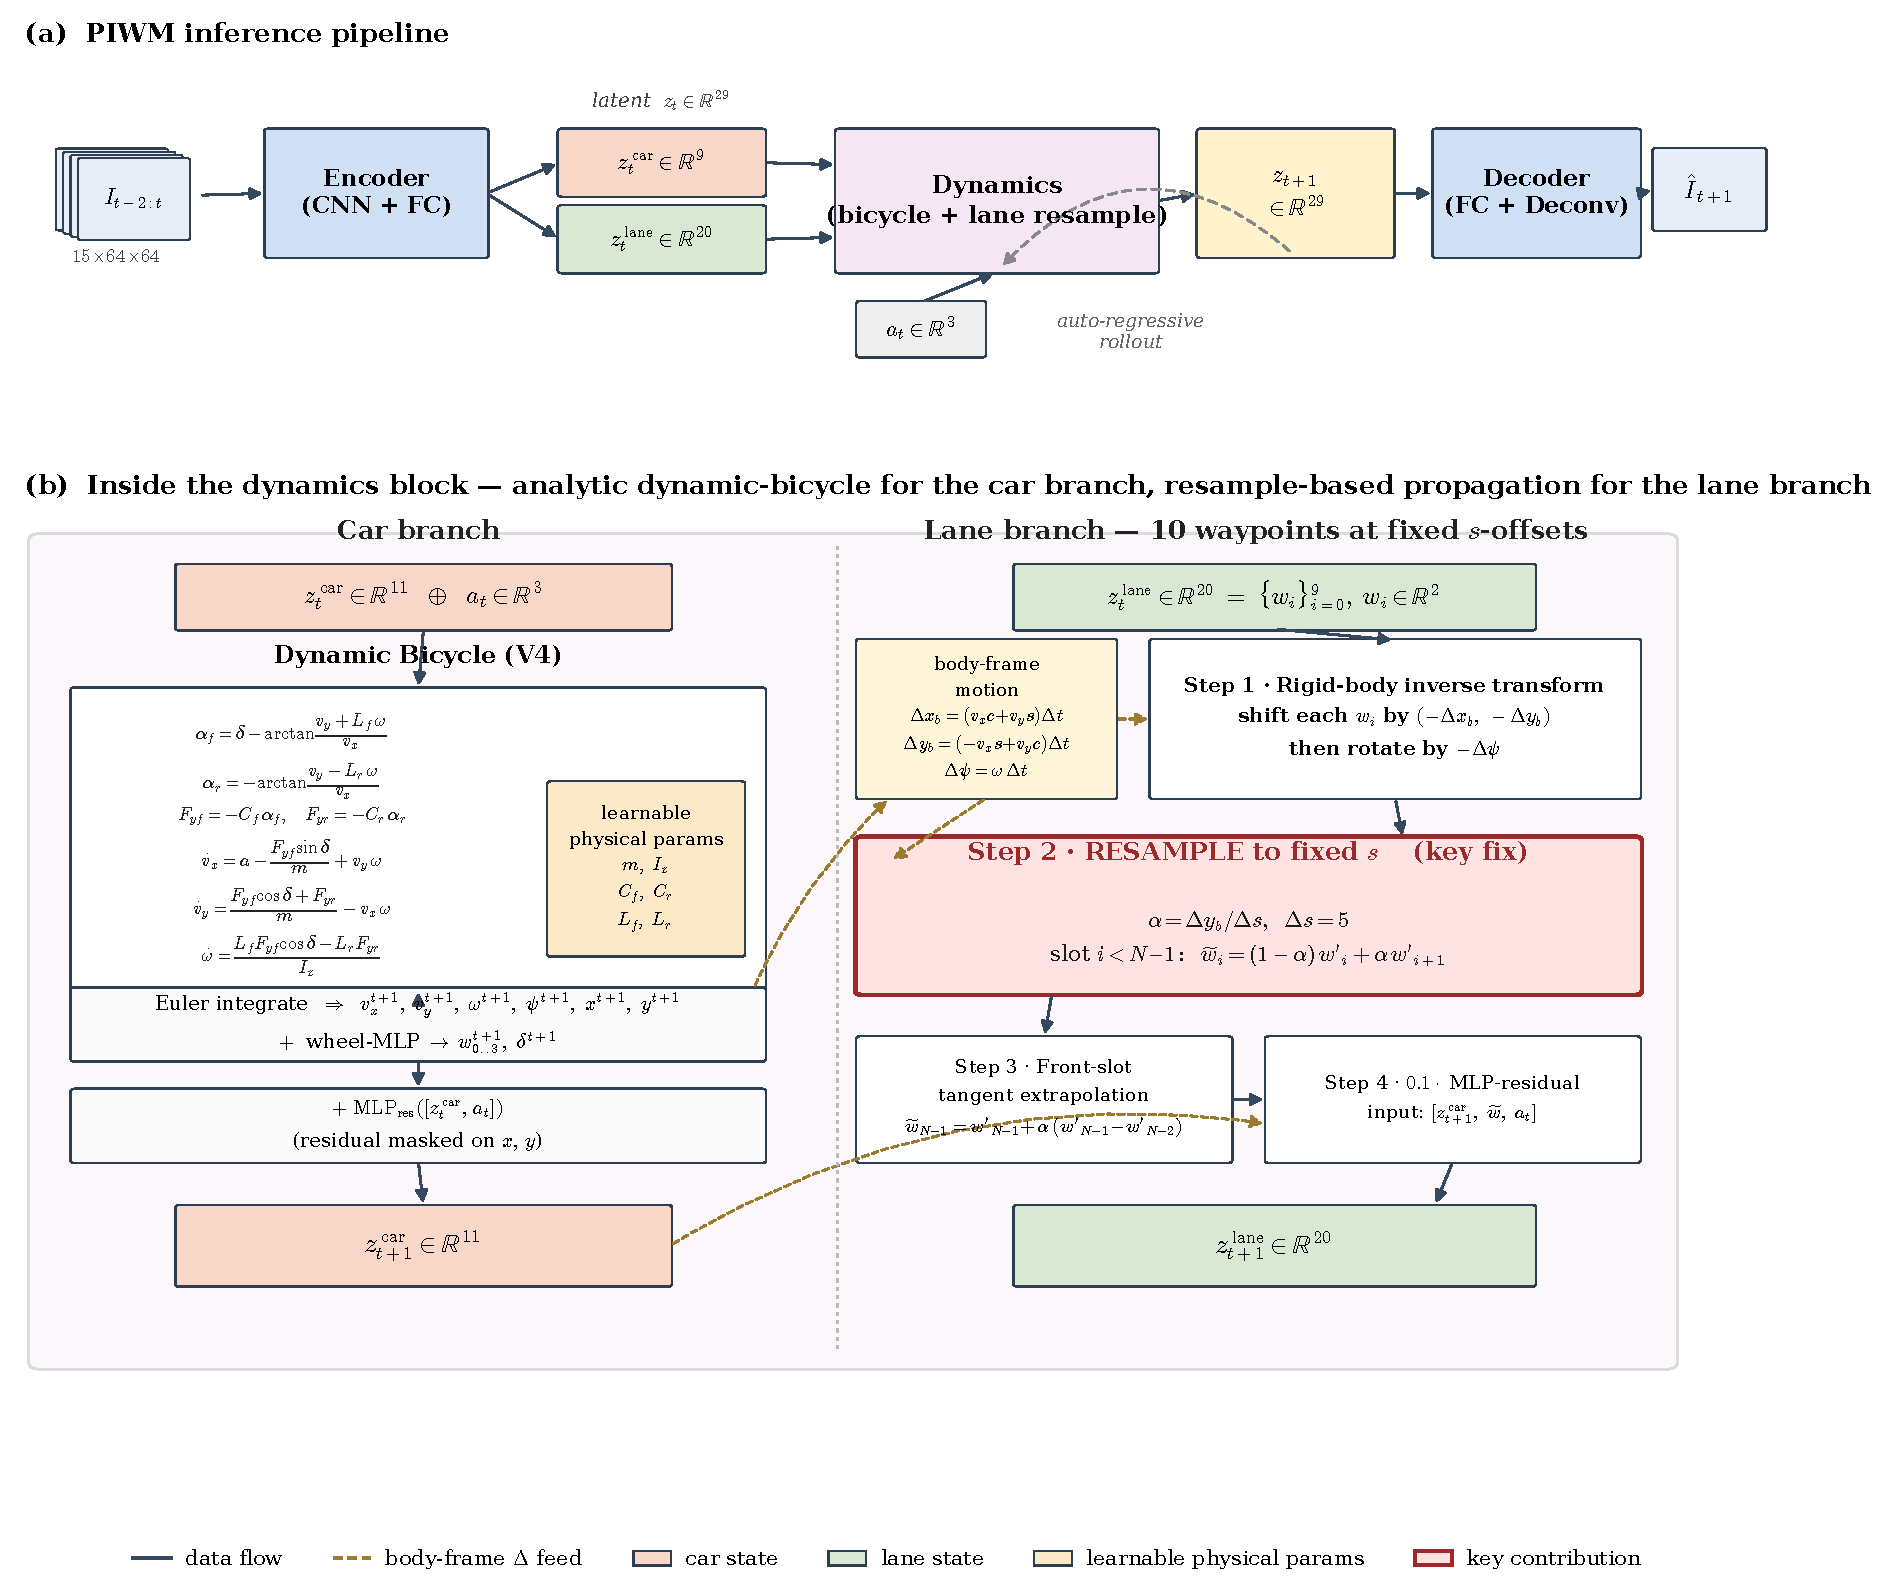
\includegraphics[width=0.95\textwidth]{../reports/figures/architecture.pdf}
    \caption{Overview of the PIWM architecture.
    A vision encoder maps observations to a visual latent; a physical encoder
    extracts the factorized interpretable state
    $\zstar = [\zv, \zr]$ (vehicle-relative state and road context); and a
    split-dynamics model rolls the state forward, applying a learnable bicycle
    kinematic model to $\zv$ and a structured, geometry-driven transition to
    $\zr$. The encoder (Section~\ref{sec:encoding}) infers the external road
    environment from images; the predictor (Section~\ref{sec:prediction})
    forecasts how that environment evolves.}
    \label{fig:arch}
\end{figure*}

\subsection{Learning Interpretable Representations}\label{sec:repr_learning}

The autoencoder maps high-dimensional observations to a physically interpretable
latent state aligned with the true physical state.
We follow the conference paper in considering two architectural approaches.

\paragraph{Intrinsic encoding.}
The encoder $\mathcal{E}: Y \rightarrow Z^*$ maps an observation directly to the
interpretable latent, partitioned as $\zstar = [z_p^*, z_v^*]$, where $z_p^*$ is
the physically interpretable component and $z_v^*$ captures the residual visual
information needed for reconstruction.
For continuous latent spaces, the objective follows a $\beta$-VAE formulation with
interpretability alignment applied to $z_p^*$:
\begin{equation}
\mathcal{L}_{\mathrm{intrinsic\text{-}cont}} =
    \mathcal{L}_{\mathrm{recon}}(y, \hat{y})
    + \lambda_{\mathrm{interp}}\,\mathcal{L}_{\mathrm{interp}}(z_p^*, \Xi)
    + \beta\, D_{\mathrm{KL}}\!\left(q(z_v^*|y)\,\|\,\mathcal{N}(0,I)\right).
\end{equation}
For discrete latent spaces, the codebook is partitioned so that each entry
$\mathbf{e}_k = [\mathbf{e}_k^p, \mathbf{e}_k^v]$ has a fixed physical component
and a learnable visual component.
The interpretability loss is applied to the averaged physical part of the
selected codebook entries.

\paragraph{Extrinsic encoding.}
The extrinsic approach decouples visual perception from physical interpretation
via a two-stage process.
In the first stage, a vision autoencoder $(\mathcal{E}_v, \mathcal{D}_v)$ is
trained on image reconstruction only, producing an intermediate latent
$z = \mathcal{E}_v(y)$.
For continuous variants this is a $\beta$-VAE; for discrete variants a VQ-VAE
with a 512-entry codebook.
In the second stage, the vision encoder is frozen and a physical encoder
$\mathcal{E}_p$ is trained to map $z$ to the interpretable state
$\zstar = \mathcal{E}_p(z)$, optimizing:
\begin{equation}
    \mathcal{L}_{\mathrm{physical}} =
    \lambda_{\mathrm{interp}}\,\mathcal{L}_{\mathrm{interp}}(\zstar, \Xi)
    + \lambda_{\mathrm{latent}}\,\mathcal{L}_{\mathrm{recon}}\!\left(z,
    \mathcal{D}_p(\zstar)\right).
\end{equation}
The physical encoder $\mathcal{E}_p$ is implemented as a Transformer over the
temporal latent sequence (Section~\ref{sec:encoding}), with mean pooling and
linear projection to the factorized state $\zstar = [\zv, \zr]$.

The conference paper's systematic comparison showed that the extrinsic approach
with a discrete (VQ) latent consistently yields the strongest physical grounding
and prediction accuracy; we adopt this configuration as the primary model for the
driving experiments.

\paragraph{Interpretability loss.}
For all variants, alignment between the encoded state and the physical variables
is enforced through the mean squared error to the empirical mean of the
supervisory samples:
\begin{equation}
    \mathcal{L}_{\mathrm{interp}}(\zstar, \Xi)
    = \left\| \zstar - \hat{\mu}_\Xi \right\|_2^2,
    \quad \hat{\mu}_\Xi = \frac{1}{L}\sum_{l=1}^L \xi^{(l)}.
    \label{eq:interp_loss}
\end{equation}
When applied to the factorized state, this loss is evaluated separately on the
vehicle-relative and road-context components with supervision from $\Xi^v$ and
$\Xi^r$:
\begin{equation}
    \mathcal{L}_{\mathrm{interp}}^{\mathrm{drive}} =
    \lambda_v\,\mathcal{L}_{\mathrm{interp}}(\zv, \Xi^v)
    + \lambda_r\,\mathcal{L}_{\mathrm{interp}}(\zr, \Xi^r).
    \label{eq:interp_loss_drive}
\end{equation}
The separate weighting of the road-context term $\lambda_r$ reflects its central
role: it is the term that forces the encoder to commit capacity to the external
environment rather than only to the vehicle.

%% --------------------------------------------------------------
\subsection{Encoding the Road Environment}\label{sec:encoding}  %% [NEW]
%% --------------------------------------------------------------

\paragraph{Challenge and motivation.}
The conference model encoded only the controlled body's state, which for the
benchmarks was directly inferable from a single frame.
Road context is different in two ways.
First, it is a property of the \emph{environment}, not the agent, so it must be
read off the scene rather than the vehicle's appearance.
Second, for a forward-facing camera it is only \emph{partially visible}: at any
instant the camera sees a limited stretch of road, and quantities such as the
curvature of the lane the vehicle is about to enter are not fully determined by
the current frame.
A single-frame encoder is therefore insufficient; the road context must be
aggregated over time.

\paragraph{Temporal road-context encoder.}
We condition the physical encoder on a history of visual latents:
\begin{equation}
    (\zv_t,\; \zr_t) = \mathcal{E}_p(z_{t-k+1:t}),
    \qquad z_{\tau} = \mathcal{E}_v(y_{\tau}),
    \label{eq:temporal_encoder}
\end{equation}
where $k$ is the context-window length.
The Transformer-based physical encoder handles variable-length temporal inputs
via self-attention, allowing it to aggregate motion and appearance cues across
frames: as the vehicle advances, the road geometry that was previously seen far
ahead becomes the geometry the vehicle is on, so a temporal window disambiguates
cross-track error, heading error, and curvature that a single frame leaves
ambiguous.
The encoder produces both components jointly but supervises them separately
through~\eqref{eq:interp_loss_drive}, ensuring $\zr_t$ carries genuine
environmental information rather than being absorbed into the vehicle component.

\paragraph{Privileged supervision for real-world deployment.}
On the real DonkeyCar, the road context cannot be measured by the deployed car
itself.
We therefore use \emph{privileged supervision}: during training, an external
localization system (a known track map together with the logged car pose, as is
also obtainable from an overhead camera) provides ground-truth road context
$\Xi^r$ for each frame; at test time this signal is withheld and the deployed car
observes only its front camera.
The encoder~\eqref{eq:temporal_encoder} is thus trained to predict, from the
onboard image stream alone, the road context that the privileged signal supplied
during training.
This is precisely a teacher--student / learning-from-privileged-information
setup~\cite{chen2020learning}: the privileged road context teaches the encoder
what to extract, and at deployment the encoder reconstructs it from images.
Because $\zr$ is physically interpretable, the recovered road context can be
inspected and compared against the true lane geometry, which we use as a
diagnostic in Section~\ref{sec:results}.

\begin{figure}[t]
    \centering
    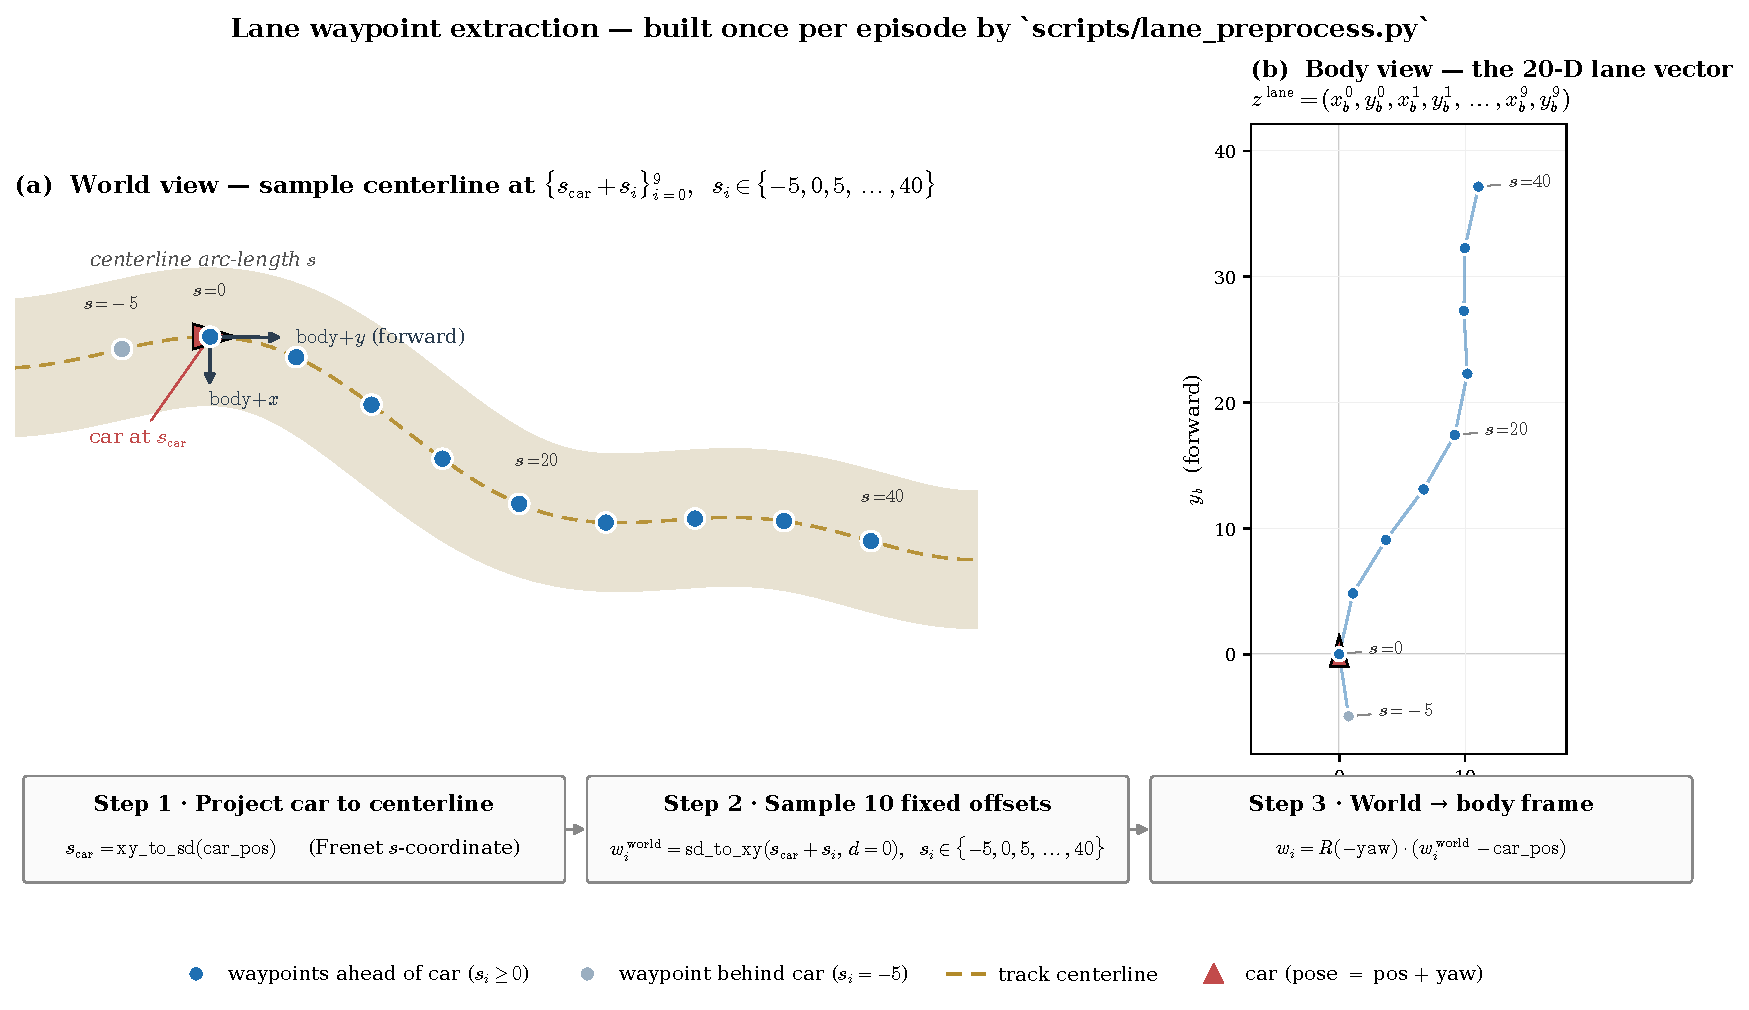
\includegraphics[width=\linewidth]{../reports/figures/lane_waypoints.pdf}
    \caption{Encoding the road environment. The road-context state $\zr$
    (cross-track error $e_{\mathrm{CTE}}$, heading error $e_\psi$, curvature
    $\kappa$) describes the lane ahead in the vehicle's body frame and is
    inferred from a temporal window of onboard images. On the real DonkeyCar this
    encoding is supervised by privileged track localization at training time and
    recovered from the front camera alone at test time.}
    \label{fig:encoding}
\end{figure}

%% --------------------------------------------------------------
\subsection{Predicting the Road Environment}\label{sec:prediction}  %% [NEW]
%% --------------------------------------------------------------

\paragraph{Challenge and motivation.}
Encoding the road at the current step is necessary but not sufficient.
To roll out a trajectory over a long horizon without new observations, the world
model must anticipate how the road context itself changes as the vehicle advances:
the curve that is ahead now is underfoot a few steps later, and the cross-track
and heading errors evolve as the vehicle tracks (or departs from) the lane.
A model that predicts only the vehicle state, holding the road context fixed or
ignoring it, drifts quickly because it steers the predicted vehicle through a road
that no longer matches reality.
We therefore make road prediction an explicit, physically interpretable part of
the dynamics.

\paragraph{Split dynamics.}
We use a \emph{split-dynamics} model that advances the vehicle and the road
context with separate, physically appropriate transitions:
\begin{align}
    \hat{\zv}_{t+1} &= \phi_\theta(\zv_t,\; a_t),
        \label{eq:split_vehicle}\\
    \hat{\zr}_{t+1} &= f_r(\zr_t,\; \zv_t,\; a_t;\; \theta_r).
        \label{eq:split_road}
\end{align}
The vehicle transition $\phi_\theta$ is the learnable bicycle kinematic model
(below); the road transition $f_r$ is a structured, geometry-driven model
(below).
Splitting the dynamics decouples the fast-varying vehicle motion from the
slow-varying road geometry and lets each receive its correct inductive bias.

\paragraph{Bicycle kinematic model for the vehicle.}
For driving environments we replace the generic second-order dynamics of the
conference paper with a \emph{bicycle kinematic model}, a physically appropriate
prior for wheeled-vehicle motion:
\begin{align}
    x_{t+1}    &= x_t    + v_t\cos(\psi_t + \beta_t)\,\Delta t,
    \label{eq:bic_x}\\
    y_{t+1}    &= y_t    + v_t\sin(\psi_t + \beta_t)\,\Delta t,
    \label{eq:bic_y}\\
    \psi_{t+1} &= \psi_t + \frac{v_t}{l_r}\sin(\beta_t)\,\Delta t,
    \label{eq:bic_psi}\\
    v_{t+1}    &= v_t    + a_t\,\Delta t,
    \label{eq:bic_v}
\end{align}
where $\beta_t = \arctan\!\left(\frac{l_r}{l_f + l_r}\tan(\delta_{f,t})\right)$
is the slip angle, $l_f$ and $l_r$ are the distances from the center of mass to
the front and rear axles, $\delta_{f,t}$ is the steering angle, $v_t$ is the
longitudinal speed, and $\psi_t$ is the heading.
The wheelbase parameters $l_f, l_r$ are unknown and learned during training.
The vehicle-relative dynamics~\eqref{eq:split_vehicle} apply
\eqref{eq:bic_x}--\eqref{eq:bic_psi} in the local frame of each window, expressing
displacements relative to the initial timestep~\eqref{eq:vehicle_rel}.

\paragraph{Structured road-context transition.}
The road-context state $(e_{\mathrm{CTE}}, e_\psi, \kappa)$ evolves slowly and
geometrically.
As the vehicle moves by the body-frame increment implied by its predicted motion,
the road ahead is effectively re-indexed: the lane geometry is advected past the
vehicle.
We therefore model $f_r$ as a geometry-driven transition that (i) updates the
cross-track error and heading error from the vehicle's predicted lateral and
angular motion relative to the road, and (ii) advances the curvature
conservatively, treating it as locally constant over a single step and updating it
toward the curvature of the next road segment:
\begin{equation}
    \zr_{t+1} = f_r(\zr_t,\; \zv_t,\; a_t;\; \theta_r).
    \label{eq:road_dyn}
\end{equation}
A small learnable residual corrects for effects not captured by the rigid
geometric update (e.g., imperfect lane tracking), with $\theta_r$ learned jointly.
Crucially, because $f_r$ operates on the physically interpretable $\zr$, the
forecasted road context at any horizon is itself interpretable: the model outputs
a predicted lane geometry that can be visualized and checked, not an opaque
feature.

\begin{figure}[t]
    \centering
    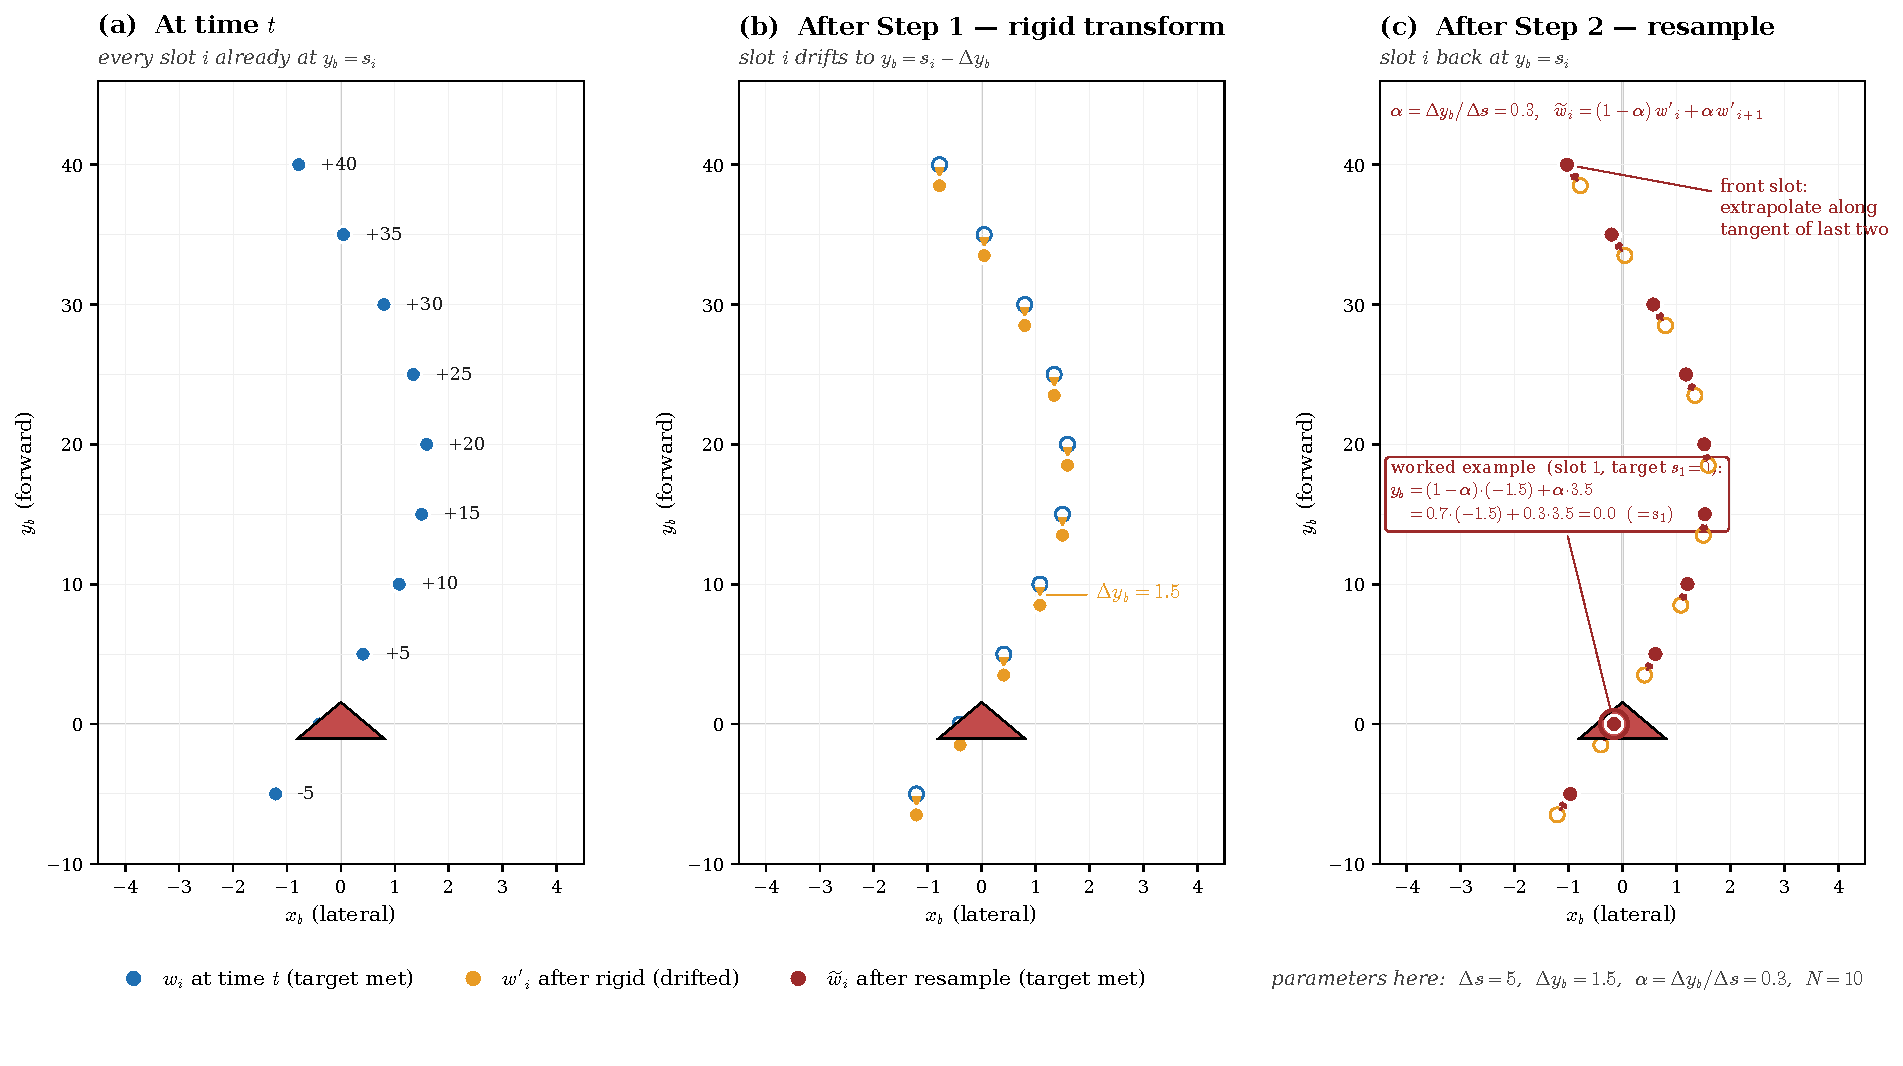
\includegraphics[width=\linewidth]{../reports/figures/lane_resample.pdf}
    \caption{Predicting the road environment. As the vehicle advances, the road
    context is advected past it: the geometry ahead is re-indexed under the
    predicted ego motion (a quasi-rigid geometric update) and corrected by a small
    learned residual. Because the predicted road context remains physically
    interpretable, the forecasted lane can be inspected at every horizon.}
    \label{fig:prediction}
\end{figure}

\subsection{Training Procedure}

Training follows a staged pipeline.
Stage~1 trains the vision autoencoder $(\mathcal{E}_v, \mathcal{D}_v)$ on image
reconstruction.
Stage~2 trains the physical encoder $\mathcal{E}_p$ to produce the factorized
interpretable state, optimizing~\eqref{eq:interp_loss_drive} jointly with a latent
reconstruction term.
Stage~3 trains the split-dynamics models ($\phi_\theta$ for the vehicle and $f_r$
for the road context), with an optional end-to-end fine-tuning pass that updates
the encoder and dynamics together to align the encoded state with what the
dynamics can predict.
Algorithm~\ref{alg:piwm_drive} summarizes the procedure.

\begin{algorithm}[t]
\caption{PIWM training for partially observable driving.}
\label{alg:piwm_drive}
\begin{algorithmic}[1]
\Require Training set $\mathcal{S}$, loss weights
         $\lambda_v, \lambda_r, \lambda_{\mathrm{dyn}}$, context length $k$
\State Train vision autoencoder $(\mathcal{E}_v, \mathcal{D}_v)$ on image
       reconstruction
\For{each batch $(y_{1:M}, a_{1:M}, \Xi^v_{1:M}, \Xi^r_{1:M})$}
    \State $z_t \gets \mathcal{E}_v(y_t)$ for all $t$
    \State $(\zv_t, \zr_t) \gets \mathcal{E}_p(z_{t-k+1:t})$
           \Comment{encode vehicle and road (Sec.~\ref{sec:encoding})}
    \State Update $\mathcal{E}_p$ with
           $\lambda_v\,\mathcal{L}_{\mathrm{interp}}(\zv_t, \Xi^v_t)
           + \lambda_r\,\mathcal{L}_{\mathrm{interp}}(\zr_t, \Xi^r_t)
           + \lambda_{\mathrm{latent}}\,\mathcal{L}_{\mathrm{recon}}$
\EndFor
\For{each batch}
    \State Obtain $(\zv_t, \zr_t)$ from the encoders
    \State $\hat{\zv}_{t+1} \gets \phi_\theta(\zv_t, a_t)$
           \Comment{bicycle model}
    \State $\hat{\zr}_{t+1} \gets f_r(\zr_t, \zv_t, a_t;\,\theta_r)$
           \Comment{road prediction (Sec.~\ref{sec:prediction})}
    \State Update $\theta$ (bicycle) and $\theta_r$ (road) on the multi-step
           rollout loss
           $\|\hat{\zv}_{t+1} - \hat{\mu}_{\Xi^v_{t+1}}\|^2
           + \|\hat{\zr}_{t+1} - \hat{\mu}_{\Xi^r_{t+1}}\|^2$
\EndFor
\State (Optional) End-to-end fine-tune $\mathcal{E}_p, \phi_\theta, f_r$ jointly
\State \Return trained model parameters
\end{algorithmic}
\end{algorithm}


%% ==============================================================
\section{Experimental Evaluation}\label{sec:experiments}
%% ==============================================================

\subsection{Environments and Evaluation Tiers}

We evaluate across three tiers of increasing difficulty.
Tier~1 establishes continuity with the conference paper; Tiers~2 and~3 are the two
new partially observable driving case studies (Contribution~1).

\paragraph{Tier~1: Fully observable benchmarks.}
\textbf{CartPole} and \textbf{Lunar Lander}~\cite{brockman2016openai} are retained
from the conference paper as controlled settings where the system state is a
complete Markov description.
These results establish continuity with the conference version and a clean
baseline for physically interpretable prediction under simple dynamics.

\paragraph{Tier~2: Partially observable simulated driving (CarRacing).}
\textbf{CarRacing}~\cite{brockman2016openai} is a top-down simulated racing
environment in which the vehicle navigates a procedurally generated track.
The observation is a bird's-eye-view RGB image (native $96 \times 96$, resized to
$64 \times 64$ for the encoder).
The vehicle's kinematic state is available from the simulator, but the road
geometry (the shape of the upcoming track and the vehicle's relationship to the
lane) is not part of the state and must be inferred from the image.
Because the camera is top-down, the road ahead is visible but the model must still
\emph{encode} it into the physical road context and \emph{predict} its evolution
during rollout.
This is the primary controlled testbed for the factorized-state formulation and
split dynamics.

\paragraph{Tier~3: Real-world DonkeyCar deployment.}
The \textbf{DonkeyCar (real)} tier evaluates the factorized formulation on a
physical RC-scale autonomous car driven on a laboratory track.
The car observes its environment through a front-facing camera (the test-time
observation, $64 \times 64$), and logs wheel-encoder speed, steering, and pose.
This is the most demanding tier: the camera is forward-facing, so the road ahead
is only partially visible, and the road context cannot be measured by the deployed
car.
We collect driving trajectories on the physical platform and derive ground-truth
road context from external track localization, used as privileged supervision at
training time only (Section~\ref{sec:encoding}); at test time the model infers and
rolls out road context from the onboard front-camera stream alone.

\subsection{Experimental Setup}\label{sec:setup}

\paragraph{Benchmarks (Tier~1).}
The data-collection and weak-supervision protocol follows the conference paper.
For each environment, we collect 60{,}000 trajectories of at least 50 steps,
generated by a mix of random actions and a pretrained neural controller.
Weak-supervision labels are synthesized by adding biased uniform noise of relative
width $\delta \in \{0\%, 5\%, 10\%\}$ to the ground-truth state, as described in
Appendix~\ref{sec:interp_loss_def}.

\paragraph{CarRacing (Tier~2).}
Driving data are generated with a pretrained controller on procedurally generated
tracks; each episode records the onboard image, action, and simulator state.
Ground-truth labels for the vehicle-relative state $(x_{\mathrm{rel}},
y_{\mathrm{rel}}, \psi_{\mathrm{rel}})$ and the road-context state
$(e_{\mathrm{CTE}}, e_\psi, \kappa)$ are available directly from the simulator and
its track geometry.
We use exact ground-truth labels for training (corresponding to $\delta = 0$) and
evaluate whether the factorized-state formulation improves long-horizon prediction
relative to baselines that use only vehicle-state labels.

\paragraph{DonkeyCar real (Tier~3).}
We drive the physical DonkeyCar on a closed laboratory track and record
synchronized front-camera frames ($64 \times 64$), control actions
(steering, throttle), and vehicle pose, at approximately \SI{22}{fps}.
Trajectories are segmented into clean contiguous laps; brief sensing artifacts
(dropped or interpolated frames, pose glitches) are filtered out before training.
Ground-truth road context is computed from the known track centerline and the
logged pose (privileged supervision), and is withheld at test time.
We hold out a subset of laps for evaluation and report prediction error on the
held-out laps.

\paragraph{Architecture and training.}
The driving experiments use the extrinsic PIWM variant (a vision encoder followed
by a Transformer physical encoder producing the factorized state), which the
conference paper showed to be the strongest configuration.
The vision encoder maps each $64 \times 64$ observation to a compact latent.
The physical encoder uses a temporal context window to infer road context from
image sequences (Section~\ref{sec:encoding}).
Dynamics are trained with a cosine learning-rate schedule and early stopping on
validation loss.
All baselines are trained under identical conditions with the same data,
optimizer (Adam), and evaluation protocol.

\subsection{Baselines}

We compare against the same families used in the conference paper, augmented with
ablations that isolate the road-context contributions.
Data-driven sequence models (\textbf{LSTM} and \textbf{Transformer}) serve as
non-physical benchmarks.
\textbf{DVBF}~\cite{karl2016deep}, \textbf{GokuNet}~\cite{linial_generative_2021},
and \textbf{Vid2Param}~\cite{asenov2019vid2param} are physics-aware baselines, and
\textbf{SindyC}~\cite{BRUNTON2016710} is a classical dynamics-discovery baseline
operating on the interpretable latent.
For driving, to isolate the contribution of road-context encoding and prediction,
we additionally include two PIWM ablations:
\textbf{PIWM-linear} (PIWM with a linear vehicle-dynamics model and no road
context) and \textbf{PIWM-bicycle} (the bicycle model on the vehicle state, again
without the road-context factorization).
The gap between these ablations and the full model measures the value of encoding
and predicting the road, not just the vehicle.

\subsection{Metrics}

The primary metric is the root mean squared error (RMSE) of the predicted state
over multi-step rollout horizons.
For benchmark tasks, RMSE is computed over all state dimensions.
For driving tasks, RMSE is evaluated on the vehicle-relative state:
\begin{equation}
    \mathrm{RMSE}_{xy} =
    \sqrt{\frac{1}{N}\sum_{i=1}^N
    \left( (\hat{x}_{\mathrm{rel},i} - x_{\mathrm{rel},i})^2
          + (\hat{y}_{\mathrm{rel},i} - y_{\mathrm{rel},i})^2
    \right)}.
\end{equation}
We additionally report the road-context prediction error (on
$e_{\mathrm{CTE}}, e_\psi, \kappa$) to evaluate the quality of the predicted road
environment directly.
We evaluate at horizons of 30 steps (benchmarks) and up to 100 steps (driving).
For environments where ground-truth physical parameters are known (CartPole,
Lunar Lander), we additionally report relative parameter-recovery error.


%% ==============================================================
\section{Results}\label{sec:results}
%% ==============================================================

\subsection{Benchmark Results (Tier~1)}\label{sec:conf_results}

The fully observable benchmark results are carried over from the conference
paper~\cite{piwm_conf} and summarized here for completeness.
Across CartPole, Lunar Lander, and DonkeyCar, the extrinsic-discrete PIWM variant
consistently achieves the lowest and most stable 30-step prediction error,
substantially outperforming data-driven and physics-aware baselines; the quantized
latent provides strong regularization that improves long-horizon stability.
PIWM also recovers the ground-truth physical parameters of CartPole and Lunar
Lander with low relative error across all noise levels $\delta$, confirming that
the learned representations are genuinely physically grounded rather than merely
correlated with the physics.
These benchmark results establish that the driving extension is a proper superset
of the original framework: on fully observable tasks, where the vehicle state is
already Markov, PIWM behaves exactly as before.

\subsection{CarRacing Results (Tier~2)}\label{sec:carracing_results}

\begin{figure*}[t]
    \centering
    
\includegraphics[width=0.95\textwidth]{../vis/final_state_mse.png}
    \caption{Prediction performance on CarRacing. State error over a 100-step
    horizon for $x_{\mathrm{rel}}$, $y_{\mathrm{rel}}$, and $\psi_{\mathrm{rel}}$,
    comparing PIWM (with factorized state and split dynamics) against PIWM-linear,
    PIWM-bicycle (vehicle state only, no road context), SindyC, GokuNet, DVBF, and
    Vid2Param. Methods that encode and predict the road context remain accurate at
    long horizons, while vehicle-only and data-driven baselines diverge.}
    \label{fig:carracing}
\end{figure*}

Figure~\ref{fig:carracing} reports state error over a 100-step prediction horizon
on CarRacing.
Table~\ref{tab:carracing} summarizes the longitudinal-displacement
($x_{\mathrm{rel}}$) error at representative horizons.

\begin{table}[t]
\centering
\caption{CarRacing longitudinal-displacement ($x_{\mathrm{rel}}$) prediction
error at increasing horizons (lower is better). PIWM with the bicycle model and
road-context factorization maintains low error to 100 steps, whereas the
vehicle-only ablations (PIWM-linear, PIWM-bicycle) and most baselines diverge.
\emph{The numerical entries are populated from our evaluation runs; confirm
against the final experiment freeze before submission.}}
\label{tab:carracing}
\small
\begin{tabular}{lrrrr}
\toprule
Model & step 20 & step 50 & step 75 & step 100 \\
\midrule
PIWM-linear            & 0.015 & 0.124 & 0.559 & 1.985 \\
PIWM-bicycle (veh.\ only) & 0.008 & 0.186 & 0.696 & 2.020 \\
SindyC                 & 0.046 & 0.927 & 4.493 & 15.03 \\
DVBF                   & 0.009 & 0.182 & 1.242 & 3.556 \\
Vid2Param              & 0.001 & 0.094 & 1.093 & 6.044 \\
GokuNet                & 0.001 & 0.038 & 0.324 & 1.405 \\
\textbf{PIWM (ours, full)} & \textbf{0.002} & \textbf{0.026} & \textbf{0.074} & \textbf{0.306} \\
\bottomrule
\end{tabular}
\end{table}

The proposed PIWM with the bicycle model and factorized state substantially
outperforms all baselines across the state dimensions and across the full 100-step
horizon.
Critically, the two ablations that drop the road context, PIWM-linear and
PIWM-bicycle (vehicle state only), are competitive at short horizons but diverge
as the horizon grows: by 75--100 steps their error is roughly an order of
magnitude larger than the full model.
This is the central empirical signature of partial observability.
A vehicle-only model cannot anticipate the upcoming road geometry, so once the
rollout enters curvature that was not represented, errors compound; the full
model, which encodes the road context and predicts its evolution, steers the
predicted vehicle through the correct geometry and stays accurate.
Data-driven baselines (LSTM-style and GokuNet) and the physics-aware DVBF and
Vid2Param exhibit rapid error growth at long horizons, consistent with the
conference findings.

\paragraph{Quality of the predicted road environment.}
Because $\zr$ is interpretable, we can inspect the forecasted road directly.
The predicted road context (cross-track error, heading error, curvature) tracks
the ground-truth lane geometry over the rollout, confirming that the model is not
merely improving vehicle prediction as a side effect but is genuinely forecasting
the external environment in physically meaningful terms.

\subsection{Real DonkeyCar Results (Tier~3)}\label{sec:donkeyreal_results}

We deploy the learned model on the physical DonkeyCar, where the road context is
supervised only during training and must be inferred from the front camera at test
time.

\paragraph{Short-horizon accuracy.}
For one-step prediction from a temporal observation context, the model attains a
relative displacement error of
$\mathrm{RMSE}_x = \SI{0.057}{m}$, $\mathrm{RMSE}_y = \SI{0.048}{m}$, and
$\mathrm{RMSE}_{xy} = \SI{0.075}{m}$, i.e.\ an average positional error of roughly
\SI{7.5}{cm} on the physical car.

\paragraph{Per-lap analysis.}
Prediction error varies across laps.
Most laps yield consistent, low error; a few exhibit larger error traceable to
sensing artifacts in the recorded trajectory (occasional pose irregularities from
logging noise) rather than model failure.
To characterize the model under clean conditions, we report a best-lap analysis:
on the best-performing lap the model attains
\[
    \mathrm{RMSE}_{xy} = \SI{0.0238}{m},
\]
roughly \SI{2.4}{cm} of positional error.
Figure~\ref{fig:donkey_bestlap} compares the predicted trajectory against the
ground-truth path for this lap; the predicted displacements closely follow the
true trajectory, demonstrating accurate motion prediction on real hardware when
the underlying data are clean.

\begin{figure}[t]
    \centering
    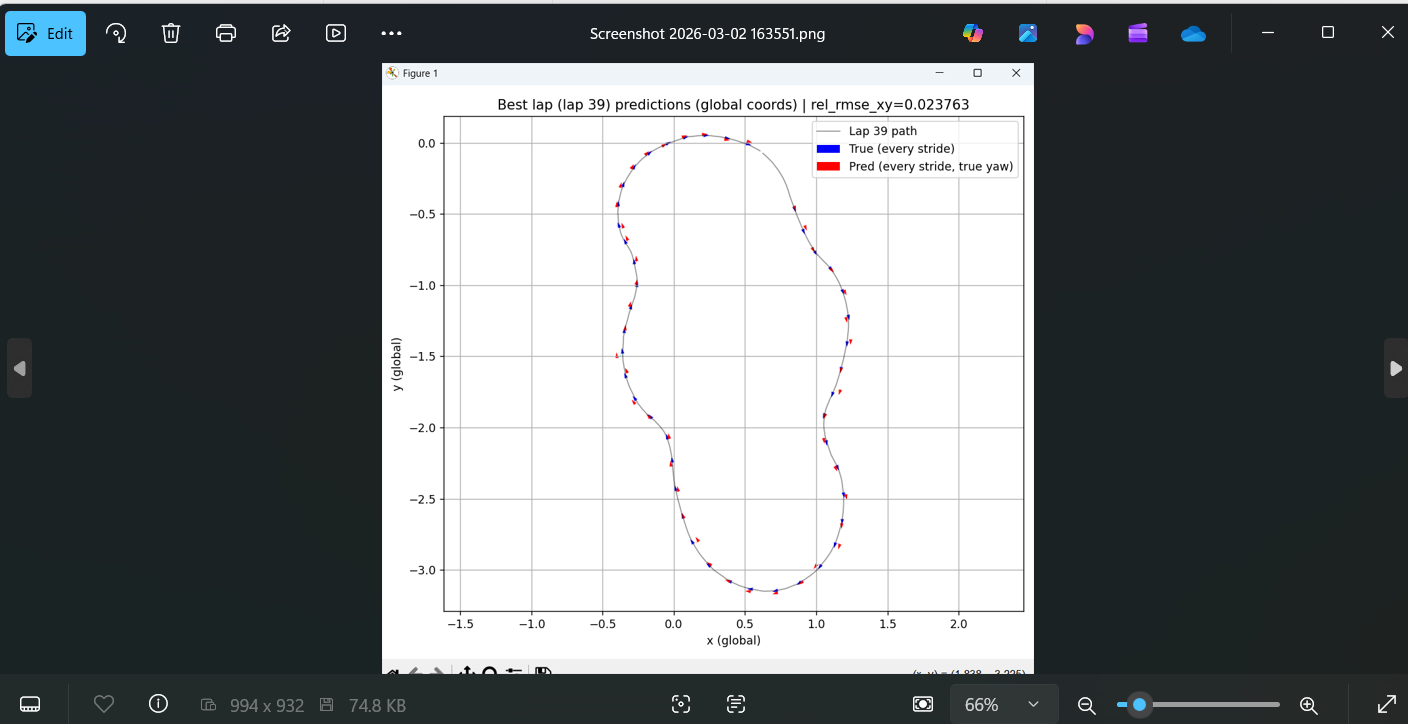
\includegraphics[width=0.8\linewidth]{donkeycarbestlap.png}
    \caption{Real DonkeyCar best-lap prediction. Predicted trajectory (in global
    coordinates) compared with the ground-truth path; the relative displacement
    error is $\mathrm{RMSE}_{xy} = \SI{0.0238}{m}$ (\(\approx\)\,\SI{2.4}{cm}).}
    \label{fig:donkey_bestlap}
\end{figure}

\paragraph{Long-horizon rollout.}
We additionally evaluate multi-step (autoregressive) rollout over complete laps,
feeding the predicted state and the control inputs back into the split-dynamics
model.
Across laps, the long-horizon $\mathrm{RMSE}_{xy}$ remains in the range
\SI{0.05}{m}--\SI{0.07}{m}, indicating that error stays bounded as the horizon
grows.
Figure~\ref{fig:donkey_rollout} shows representative long-horizon predictions and
the predicted lane overlaid on the ground-truth track.
The trajectories remain well aligned over most of the lap, with the largest
deviations appearing in high-curvature segments, where small per-step errors
accumulate; nonetheless the predicted road context keeps the rollout physically
plausible.
This is the key real-world finding: a factorized representation whose road context
is learned under privileged supervision transfers to deployment, where the road
must be recovered from the onboard camera alone.

\begin{figure}[t]
    \centering
    \begin{subfigure}{0.49\linewidth}
        
\includegraphics[width=\linewidth]{../figures/fig_rollout_trajectory.png}
        \caption{Long-horizon rollout.}
    \end{subfigure}
    \hfill
    \begin{subfigure}{0.49\linewidth}
        
\includegraphics[width=\linewidth]{../figures/fig_lane_overlay.png}
        \caption{Predicted vs.\ true lane.}
    \end{subfigure}
    \caption{Real DonkeyCar long-horizon behavior. (a) Predicted vs.\
    ground-truth trajectory over a lap. (b) The predicted road context (lane
    geometry) overlaid on the true lane, showing that the model forecasts the
    external environment, not only the vehicle.}
    \label{fig:donkey_rollout}
\end{figure}


%% ==============================================================
\section{Discussion}\label{sec:discussion}
%% ==============================================================

\paragraph{Encoding and predicting the road is what restores long-horizon
accuracy.}
The CarRacing results show a clear and growing gap between models that include the
road-context factorization and those that do not: vehicle-only ablations match the
full model at short horizons but diverge by 50--100 steps
(Table~\ref{tab:carracing}).
This is the empirical content of the partial observability argument from
Section~\ref{sec:problem}.
Vehicle state alone is non-Markov; the road context carries the missing
information about upcoming geometry, and both \emph{encoding} it from images and
\emph{predicting} its evolution are required for stable rollout.

\paragraph{Bicycle dynamics vs.\ generic dynamics.}
The advantage of the bicycle model over a generic linear predictor indicates that
the physical inductive bias is beneficial beyond raw capacity: the bicycle model
constrains predicted motion to physically plausible, heading-consistent
trajectories, which reduces error accumulation over long horizons.
This parallels the conference finding for benchmark tasks, where structured
dynamics outperformed black-box sequence models.

\paragraph{Interpretability of the forecasted environment.}
Because the road context is physically interpretable, the forecasted road, not
just the forecasted vehicle, can be inspected and monitored.
On both CarRacing and the real DonkeyCar, the predicted lane geometry can be
compared against ground truth, providing a diagnostic that opaque world models do
not offer.
This is directly useful for safety monitoring: a forecasted road that departs from
plausible geometry is a detectable failure signal.

\paragraph{Privileged training for real deployment.}
The real DonkeyCar uses privileged road-context supervision at training and
withholds it at test.
This reflects practical deployability: external localization (a mapped track, or
an overhead view) is available in instrumented training environments but not on a
freely deployed car.
The model must therefore learn to read road context from onboard images, guided
during training by the privileged signal.
The fact that the learned encoding transfers to the unaided setting is what makes
the approach viable on real hardware.

\paragraph{Limitations.}
First, the road-context variables are specified manually for each environment; a
more general approach might discover the decomposition automatically.
Second, the bicycle model is a kinematic approximation that ignores tire dynamics
and slip, which may limit accuracy at high speeds or on low-friction surfaces.
Third, privileged supervision requires an instrumented training environment to
obtain ground-truth road context; reducing this requirement (e.g., via
self-supervised road estimation) is open.
Finally, the method currently assumes a single vehicle and a single lane;
multi-agent and multi-lane settings are future work.

\paragraph{Future directions.}
Natural next steps include scaling PIWM to open-world driving with richer road
topology, multiple agents, and additional sensor modalities (LiDAR, radar);
treating other vehicles as additional interpretable road-context variables to
handle interactions and occlusions; and discovering the road-context structure
from data via symbolic regression or causal structure learning, which would
reduce the need for environment-specific design.


%% ==============================================================
\section{Conclusion}\label{sec:conclusion}
%% ==============================================================

This article extended the Physically Interpretable World Model (PIWM) from fully
observable benchmarks to partially observable driving.
The central observation is that driving is partially observable: the vehicle's
physical state alone is non-Markov with respect to future trajectory, because the
road context (lane geometry and the vehicle's relationship to it) is absent from
any standard state representation and only partially visible to an onboard camera.
We addressed this along three axes.
We introduced two partially observable driving case studies, a simulated
CarRacing track and a real physical DonkeyCar.
We introduced a physically interpretable \emph{encoding} of the road environment,
factorizing the interpretable state into a vehicle-relative component and a
road-context component inferred from images, including under privileged
supervision for real-world deployment.
And we introduced a physically interpretable \emph{prediction} of the road
environment, a split-dynamics model that forecasts how the road context evolves
alongside a learnable bicycle model for the vehicle.
Experiments on CarRacing and the real DonkeyCar confirm that encoding and
predicting the external environment, not merely the vehicle, is what enables
stable long-horizon prediction under partial observability, while the original
benchmark results are retained unchanged.
Physically interpretable world modeling for driving thus requires aligning latent
representations with physical variables \emph{and} decomposing those
representations according to the semantic structure of the task, so that the
external environment is both encoded and predicted in physically meaningful terms.


%% ==============================================================
\section*{Acknowledgements}
%% ==============================================================

The authors thank Liam (Cade) McGlothlin and Vedansh Maheshwari for their help in
exploring interpretable world models.
This material is based upon work supported by the U.S.\ National Science Foundation
under Grant Numbers CNS~2513076 and CCF~2403616.
Any opinions, findings, and conclusions expressed in this material are those of the
authors and do not necessarily reflect the views of the NSF.


%% ==============================================================
\appendix
\section{Weak Supervision Noise Model}\label{sec:interp_loss_def}
%% ==============================================================

The weak supervision in Tier~1 benchmark experiments follows the noise model from
the conference paper.
For the $i$-th state component with valid range size $\mathcal{X}_i$, we generate a
randomly shifted center $\tilde{\mu}_i = x_i + \Delta_i$,
$\Delta_i \sim \mathrm{Unif}[-\frac{1}{2}\delta|\mathcal{X}_i|,
\frac{1}{2}\delta|\mathcal{X}_i|]$, and draw the supervisory distribution as
$p_i(x) = \mathrm{Unif}[\tilde{\mu}_i - \frac{1}{2}\delta|\mathcal{X}_i|,\;
\tilde{\mu}_i + \frac{1}{2}\delta|\mathcal{X}_i|]$.
At each timestep, $L = 50$ samples are drawn to form the proxy supervision set
$\Xi_t$.
For Tier~2 and Tier~3 experiments, exact ground-truth labels are used at training
time ($\delta = 0$), reflecting the availability of simulator state and
training-time track localization; at test time, the road context is withheld and
inferred from images.

\bibliographystyle{elsarticle-num}
\bibliography{sample-base}

\end{document}
